% document type
\documentclass[12pt]{article}

% packages
\usepackage{amsmath} % for mathematical symbols and environments
\usepackage{amsfonts} % for additional math fonts
\usepackage{amssymb} % for additional math symbols
\usepackage{hyperref} % for hyperlinks

\usepackage{tikz} % for graphics
\usetikzlibrary{arrows,shapes}

% title and author
\title{Numeric to Symbolic to Parametric space of solutions of Polynomial Systems of Equations}
\author{Ilay Menahem}

% article text
\begin{document}

\maketitle

% abstract
\begin{abstract}
    This paper presents a working pipeline for solving polynomial systems of equations, starting from numerical solutions using Newton-Raphson method, transitioning to symbolic solutions through PSLQ, and finally exploring the space of solutions. 
\end{abstract}

\section*{Introduction}
% introduction of the importance and history of polynomial systems of equations

% classic methods for solving polynomial systems of equations

\section*{Mathematical Background}
Let $\mathbb{K}[\mathbf{x}]$ denote the polynomial ring in variables $\mathbf{x} = (x_1, \ldots, x_n)$ over a field $\mathbb{K}$, typically $\mathbb{R}$ or $\mathbb{C}$. A polynomial system is defined by a map $F: \mathbb{K}^n \to \mathbb{K}^m$ with components $f_1, \ldots, f_m \in \mathbb{K}[\mathbf{x}]$. The locus of simultaneous solutions constitutes the \textit{affine variety} $V(F) = \{ \mathbf{a} \in \mathbb{K}^n \mid F(\mathbf{a}) = \mathbf{0} \}$.


\section*{Identification of elegant solutions}
there are a few ways to interpret the meaning of the solution to a polynomial system of equations.
\begin{list}{-}{}
    \item \textbf{numerical solutions:} specific numerical values for the variables that satisfy all equations in the system (with very high precision).
    \item \textbf{symbolic solutions:} specific symbolic expressions of constants that satisfy all equations in the system.
    \item \textbf{lowest norm solution:} a solution numerical or symbolic, that minimizes some norm, such as the Zero norm.
    \item \textbf{parametric expression of a variety:} a set of symbolic expressions that provide a parametric representation of the set of all possible solutions to the system, also known as the variety. it's not always possible to express the variety in a parametric form such as in the case of elliptic curves.
    \item \textbf{point cloud sampling of the variety:} a large set of numerical or symbolic solutions that sample the variety, which can be used to understand its structure and properties.
\end{list}

something of note, if one has one solution to any system of equations, one can derive a neighborhood of solutions around that point by going in the direction that is in the solution space of the Jacobian. a more in depth treatment of this idea is provided in the appendix.

\section*{Moving between types of solutions}
one can note that it is fairly straightforward to find certain types of solutions such as numerical solutions via Newton-Raphson, but sometimes it is more desirable to have symbolic solutions or parametric expressions of the variety. in the diagram below, we illustrate the different types of solutions and the methods we will use to move between them.

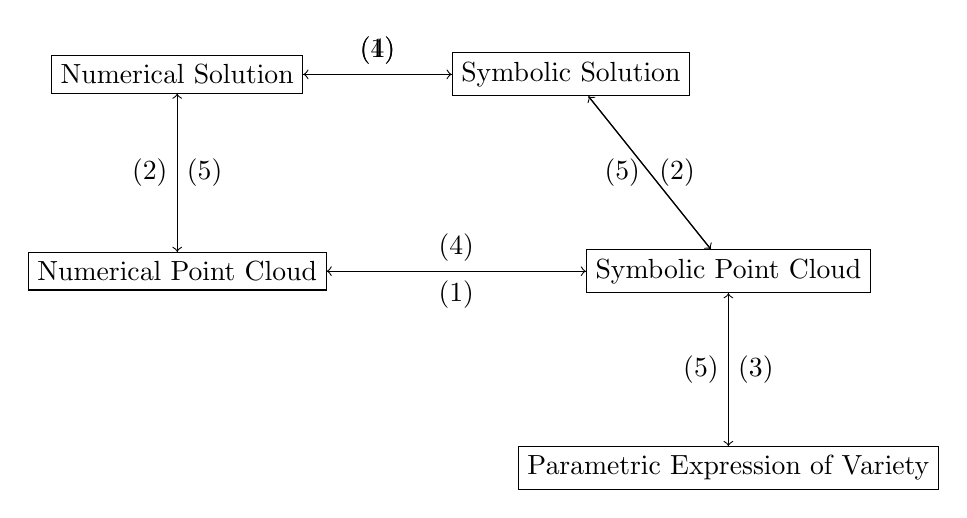
\begin{tikzpicture}
    % Define nodes
    \node[draw, rectangle] at (0, -2.5) (numerical) {Numerical Solution};
    \node[draw, rectangle] at (5, -2.5) (symbolic) {Symbolic Solution};
    \node[draw, rectangle] at (0, -5) (numerical point cloud) {Numerical Point Cloud};
    \node[draw, rectangle] at (7, -5) (symbolic point cloud) {Symbolic Point Cloud};
    \node[draw, rectangle] at (7, -7.5) (parametric) {Parametric Expression of Variety};

    % Draw arrows
    \draw[->] (numerical) -- (symbolic) node[midway, above] {(1)};
    \draw[->] (symbolic) -- (numerical) node[midway, above] {(4)};
    \draw[->] (numerical) -- (numerical point cloud) node[midway, left] {(2)};
    \draw[->] (symbolic) -- (symbolic point cloud) node[midway, right] {(2)};
    \draw[->] (numerical point cloud) -- (numerical) node[midway, right] {(5)};
    \draw[->] (symbolic point cloud) -- (symbolic) node[midway, left] {(5)};
    \draw[->] (numerical point cloud) -- (symbolic point cloud) node[midway, below] {(1)};
    \draw[->] (symbolic point cloud) -- (numerical point cloud) node[midway, above] {(4)};
    \draw[->] (symbolic point cloud) -- (parametric) node[midway, right] {(3)};
    \draw[->] (parametric) -- (symbolic point cloud) node[midway, left] {(5)};
\end{tikzpicture}

\begin{enumerate}
    \item \textbf{PSLQ:}
    \item \textbf{Going penpendicular to Jacobian null space:}
    \item \textbf{Symbolic regression:} 
    \item \textbf{Evaluating symbolic expressions:}
    \item \textbf{Sampling points:}
\end{enumerate}


\section*{Linear elimination}

even in the case of very large non linear polynomial systems of equations, it is possible to eliminate variables in a linear fashion in the following way:
\textbf{input:} polynomial system of equations $P = \{p_1, p_2, \ldots, p_k\} \subseteq \mathbb{K}[x_1, x_2, \ldots, x_m]$.
\textbf{output:} a polynomial system of equations $Q = \{q_1, q_2, \ldots, q_k\}$, which is equivalent to $P$, and each $q_i$ is a not linear in any variable $x_j$ for $j \in \{1, 2, \ldots, m\}$.
\textbf{algorithm:}
\begin{enumerate}
    \item Let $L = \{(x_j, p_i) | p_i \text{ is linear in } x_j\}$ be the list of all variables and polynomials that are linear in those variables.
    \item Let $V = \{x_1, x_2, \ldots, x_m\}$ be the set of all variables.
    \item Let $Q = P$ be the output polynomial system of equations.
    \item While $L$ is not empty:
    \begin{enumerate}
        \item Select a variable-polynomial pair $(x_j, p_i)$ from $L$.
        \item Remove $(x_j, p_i)$ from $L$, $x_j$ from $V$, and $p_i$ from $Q$.
        \item Solve $p_i$ for $x_j$: $x_j = f(\hat{x})$.
        \item For each polynomial $p_k$ in $Q$ substitute $x_j$ with $f(\hat{x})$.
        \item Update $L$ to reflect the changes in $Q$.
    \end{enumerate}
\end{enumerate}

in the example below, we demonstrate that for systems of low degree polynomials, this method can significantly reduce the number of variables and equations in the system, without increasing the degree of any polynomial in the system.

\section*{Numerical solutions via Newton-Raphson}

\section*{Symbolic solutions via iterations of PSLQ and Newton-Raphson}

\section*{exploration of space of solutions}
\subsection*{Numerical exploration of space of solutions}

\subsection*{Sybolic exploration of space of solutions}

\section*{Appendix}
\subsection*{Derivation of neighborhood of solutions via Jacobian null space}
\textbf{theorem:} let $F = \{f_1, f_2, \ldots, f_n\}$ be a system of smooth functions in variables $x = (x_1, x_2, \ldots, x_m)$. let $J$ be the Jacobian matrix of $F$ with respect to $x$, $x_0$ be a point such that $F(x_0) = 0$, and $v \in N(J(x_0))$ be a vector in the null space of $J$ at point $x_0$. 
then $\frac{d}{dt}F(x_0 + tv)|_{t=0} = 0$.

\textbf{proof:} 
By the multivariable chain rule, the derivative of the composition $F(x_0 + tv)$ with respect to $t$ is given by:
\[
\frac{d}{dt}F(x_0 + tv) = J(x_0 + tv) \cdot \frac{d}{dt}(x_0 + tv) = J(x_0 + tv) \cdot v
\]
Evaluating this expression at $t=0$:
\[
\frac{d}{dt}F(x_0 + tv)\bigg|_{t=0} = J(x_0) \cdot v
\]
Since $v$ is in the null space of $J(x_0)$, we have $J(x_0)v = 0$. Thus:
\[
\frac{d}{dt}F(x_0 + tv)\bigg|_{t=0} = 0
\]

now to an example system of polynomial equations:
\begin{align*}
f_1 &= x^2 + y^2 + z^2 - 1 = 0 \\
f_2 &= x + y + z - 1 = 0
\end{align*}
Let us choose a solution $x_0 = (1, 0, 0)$. We can verify that $f_1(1,0,0) = 1^2 + 0 + 0 - 1 = 0$ and $f_2(1,0,0) = 1 + 0 + 0 - 1 = 0$.

The Jacobian matrix $J$ is given by:
\[
J = \begin{pmatrix}
\frac{\partial f_1}{\partial x} & \frac{\partial f_1}{\partial y} & \frac{\partial f_1}{\partial z} \\
\frac{\partial f_2}{\partial x} & \frac{\partial f_2}{\partial y} & \frac{\partial f_2}{\partial z}
\end{pmatrix} = \begin{pmatrix}
2x & 2y & 2z \\
1 & 1 & 1
\end{pmatrix}
\]
Evaluating $J$ at $x_0 = (1, 0, 0)$:
\[
J(x_0) = \begin{pmatrix}
2 & 0 & 0 \\
1 & 1 & 1
\end{pmatrix}
\]
To find the null space, we solve $J(x_0)v = 0$ for $v = (v_x, v_y, v_z)^T$:
\[
\begin{pmatrix}
2 & 0 & 0 \\
1 & 1 & 1
\end{pmatrix} \begin{pmatrix}
v_x \\ v_y \\ v_z
\end{pmatrix} = \begin{pmatrix}
0 \\ 0
\end{pmatrix}
\]
From the first row, $2v_x = 0 \implies v_x = 0$.
From the second row, $v_x + v_y + v_z = 0 \implies 0 + v_y + v_z = 0 \implies v_y = -v_z$.
Let $v_z = 1$, then $v_y = -1$. Thus, a vector in the null space is $v = (0, -1, 1)^T$.

Moving from $x_0$ in the direction of $v$ keeps the system approximately solved to the first order. moving the direction of $v$ can be done numerically by choosing a small $t$, evaluating $x(t) = x_0 + tv$, and doing a Newton-Raphson step to refine the solution.

To perform the symbolic walk, we calculate the null space of $J$ symbolically. The null space direction $v(x,y,z)$ must satisfy $J v = 0$, which means $v$ is orthogonal to the gradients of $f_1$ and $f_2$. This direction is given by the cross product of the gradients (ignoring the scalar factor 2 from $\nabla f_1$):
\[
v(x,y,z) = \frac{1}{2}\nabla f_1 \times \nabla f_2 = \begin{pmatrix} x \\ y \\ z \end{pmatrix} \times \begin{pmatrix} 1 \\ 1 \\ 1 \end{pmatrix} = \begin{pmatrix} y-z \\ z-x \\ x-y \end{pmatrix}
\]
This yields the system of differential equations:
\begin{align*}
\dot{x} &= y - z \\
\dot{y} &= z - x \\
\dot{z} &= x - y
\end{align*}
Solving this system with initial condition $x(0) = (1, 0, 0)$ yields the parametric solution for the variety.

Adding the three equations gives $\dot{x} + \dot{y} + \dot{z} = 0$, implying $x+y+z = C_1$. From the initial condition, $1+0+0=1$, so $x+y+z=1$.
Differentiating $\dot{x}$ gives $\ddot{x} = \dot{y} - \dot{z} = (z-x) - (x-y) = z+y-2x$. Substituting $y+z = 1-x$, we get $\ddot{x} = (1-x) - 2x = 1 - 3x$.
This is a linear ODE $\ddot{x} + 3x = 1$. The homogeneous solution is $A\cos(\sqrt{3}t) + B\sin(\sqrt{3}t)$, and the particular solution is $x_p = 1/3$.
So $x(t) = A\cos(\sqrt{3}t) + B\sin(\sqrt{3}t) + 1/3$.
Using $x(0)=1$, we get $A + 1/3 = 1 \implies A = 2/3$.
Using $\dot{x}(0) = y(0)-z(0) = 0$, we get $\sqrt{3}B = 0 \implies B=0$.
Thus $x(t) = \frac{2}{3}\cos(\sqrt{3}t) + \frac{1}{3}$.
By symmetry and the cyclic nature of the equations, the solutions for $y$ and $z$ are phase-shifted or can be derived similarly.
Since $\dot{x} = y-z$ and $y+z = 1-x$, we have a system for $y,z$:
$y-z = -\frac{2}{\sqrt{3}}\sin(\sqrt{3}t)$ and $y+z = 1 - (\frac{2}{3}\cos(\sqrt{3}t) + \frac{1}{3}) = \frac{2}{3} - \frac{2}{3}\cos(\sqrt{3}t)$.
Adding these: $2y = \frac{2}{3} - \frac{2}{3}\cos(\sqrt{3}t) - \frac{2}{\sqrt{3}}\sin(\sqrt{3}t) \implies y(t) = \frac{1}{3} - \frac{1}{3}\cos(\sqrt{3}t) - \frac{1}{\sqrt{3}}\sin(\sqrt{3}t)$.
Subtracting: $2z = \frac{2}{3} - \frac{2}{3}\cos(\sqrt{3}t) + \frac{2}{\sqrt{3}}\sin(\sqrt{3}t) \implies z(t) = \frac{1}{3} - \frac{1}{3}\cos(\sqrt{3}t) + \frac{1}{\sqrt{3}}\sin(\sqrt{3}t)$.

The parametric solution is:
\begin{align*}
x(t) &= \frac{1}{3} + \frac{2}{3}\cos(\sqrt{3}t) \\
y(t) &= \frac{1}{3} - \frac{1}{3}\cos(\sqrt{3}t) - \frac{1}{\sqrt{3}}\sin(\sqrt{3}t) \\
z(t) &= \frac{1}{3} - \frac{1}{3}\cos(\sqrt{3}t) + \frac{1}{\sqrt{3}}\sin(\sqrt{3}t)
\end{align*}



\end{document}